\subsection{Motivation}
Metal routing is a critical step in systems integration process, where each source is connected to its fan-outs using non-crossing metal. Routing in a modern chip, with millions or even billions of transistors, can be very complicated and cumbersome, so the manufacture process has moved to automatic routing. 

Automatic routing is a very vast field, with several techniques being developed through time. Automatic routing involves lots of problems like finding shortest non-blocked path and VIAs in multi-layer routing. 

Automatic routing techniques are always a trade-off between optimality and speed. Some techniques target execution time by reaching a sub-optimal solution. Others target optimal solution with very high execution time.

In this work, we seek a good balance between performance and optimality of solution by introducing the usage of A* search for automatic routing with a modified cost function.

\subsection{Formulation}
\begin{figure}[hp]
    \centering
    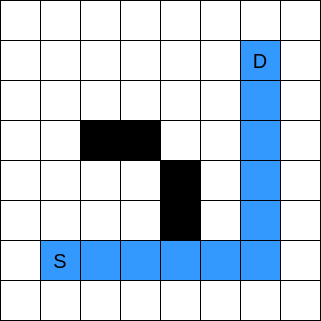
\includegraphics[width=0.4\textwidth]{figures/grid.png}
    \caption{Example of occupancy grid map (OGM), where S is the source, D is the destination, white cells aren't occupied, black cells are occupied and blue cells represent the path.}
    \label{fig:grid}
\end{figure}

Routing is formulated as a grid search problem \ref{fig:grid}, where an occupancy grid map \emph{(OGM)} is provided with some source and destination cells to be joined. The \emph{OGM} cells can have the value of $1$ for occupied cell or $0$ for empty cell. The \emph{OGM} can be of multiple levels, in case of multi-layer routing, where the cell can have a third value to indicate that the cell can be used as a VIA. Only 4-neighbor cells are considered, so the path can move up, down, left or right. The path can also move from one level to another through VIA cells.

Given that problem formulation, several grid search and shortest path algorithms can be used to find the optimal path between each source and its given destinations. These algorithms can vary based on optimality and performance.

The two main metrics considered in this work are path length and execution time. Path length between each source and destination cell is used as a measure of solution optimality. It's defined as the number of grid cells that lies on the deduced path.

Execution time is used as a measure of algorithm performance. It's simply the total elapsed time by the algorithm to find all required paths.

\subsection{Baseline}
To measure the validity and performance of our proposed method, three main baselines are used. These baselines are well-established algorithms that are currently used in industry.

\subsubsection{Maze Routing (Lee's Algorithm)}

\subsubsection{Mikami-Tabuchi’s Algorithm}

\subsubsection{TBD}

\subsection{Modified A* Search}
\begin{figure}[hp]
    \centering
    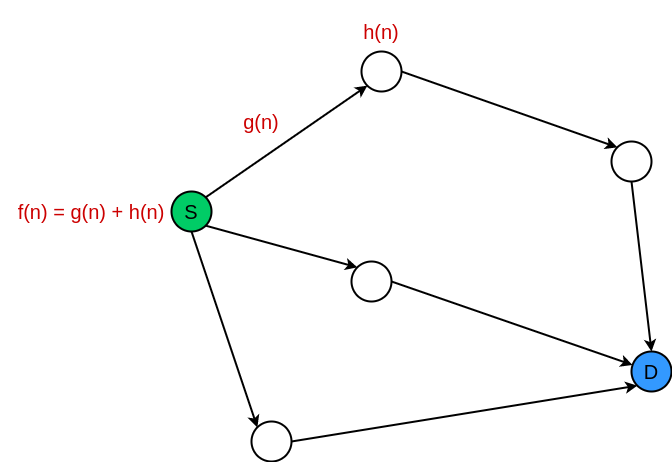
\includegraphics[width=0.4\textwidth]{figures/a_star.png}
    \caption{An illustrative example for A* search process and cost function.}
    \label{fig:astar}
\end{figure}

The main contribution of this paper is the usage of \emph{A* search} as a new routing technique. The main idea of \emph{A* search}, as shown in fig.\ref{fig:astar}, is the usage of some heuristic function to assign a cost for each node. To define a path from a source node to a destination node, the nodes that minimizes the estimated path cost are chosen at each step. The main objective is to minimize the following function:

\begin{equation} \label{eq:astar}
f(n) = g(n) + h(n)
\end{equation}
Where \emph{f(n)} is the total cost of the path from a specific node, \emph{g(n)} is the cost of the edge between current node and next chosen node and \emph{h(n)} is the estimated cost of the next chosen node based on the used heuristic function.

Thus, the required information to solve an \emph{A* search} problem is the cost of edge between each two nodes and the heuristic function to get an estimated cost for each node.

\begin{figure}[hp]
    \centering
    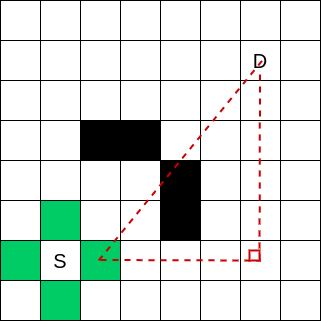
\includegraphics[width=0.4\textwidth]{figures/grid_euclid.png}
    \caption{An illustrative example for the new heuristic function based on Euclidean distance.}
    \label{fig:euclid}
\end{figure}

The \emph{OGM} representation of the routing problem can be formulated to become an \emph{A* search}. The edge cost \emph{g(n)} is always $1$, as the path can only move from one cell to an adjacent cell. The heuristic function, proposed in this work, is \emph{Euclidean distance} between next chosen cell and destination cell, as shown in  fig.\ref{fig:euclid}. So, the cost of taking any of the adjacent cells is \emph{Euclidean distance} $+$ $1$, which can be simplified to \emph{Euclidean distance} between an adjacent cell and destination cell.\\

The proposed algorithm can be summarized as follows:

\begin{algorithm}[]
\SetAlgoLined
\KwResult{Optimal path between source and destination cells.}
 append source cell to the path\;
 \While{destination not reached}{
  get adjacent cell that minimizes euclidean distance\;
  append cell to the path\;
  \If{current cell is blocked}{
   remove current cell from path\;
   backtrack to the previous cell\;
   continue\;
   }
 }
 \caption{Modified A* Search For Automatic Routing}
\end{algorithm}
